\subsection{Value Iteration \points{6}}

In this question you will carry out value iteration by hand to solve a maze. A map of the maze is shown in the table below, where `G' represents the goal of the agent (it's the terminal state); `H' represents an obstacle; the zeros are the state values V(s) that are initialized to zero.

\begin{table}[H]
\begin{center}
  \begin{tabular}{ | c | c | c | }
    \hline
    0 & 0 & G\\ \hline
    H & 0 & H \\ \hline
    0 & 0 & 0 \\ \hline
  \end{tabular}
 \caption{Map of the maze}
\end{center}
\end{table}

The agent can choose to move up, left, right, or down at each of the 6 states (the goal and obstacles are not valid initial states, ``not moving" is not a valid action). The transitions are deterministic, so if the agent chooses to move left, the next state will be the grid to the left of the previous one. However, if it hits the wall (edge) or obstacle (H), it stays in the previous state. The agent receives a reward of -1 whenever it takes an action. The discount factor $\gamma$ is 1.
 
\begin{enumerate}
\item \textbf{[1 points]} How many possible deterministic policies are there in this environment, including both optimal and non-optimal policies?

\begin{tcolorbox}[fit,height=3cm, width=\linewidth, blank, borderline={1pt}{-2pt},nobeforeafter]
    %solution
\end{tcolorbox}


\newpage

\item \textbf{[3 points]} Compute the state values after each round of synchronous value iteration updates on the map of the maze before convergence. For example, after the first round, the values should look like this:

\begin{table}[H]
\begin{center}
  \begin{tabular}{ | c | c | c | }
    \hline
    -1 & -1 & G\\ \hline
    H & -1 & H \\ \hline
    -1 & -1 & -1 \\ \hline
  \end{tabular}
 \caption{Value function after round 1}
\end{center}
\end{table}

\begin{tcolorbox}[fit,height=3.5cm, width=\linewidth, blank, borderline={1pt}{-2pt},nobeforeafter]
    %solution
    % \bgroup % Begin group for arraystretch
    \def\arraystretch{1.5}
    
    \begin{table}[H]
    \begin{minipage}{.3\linewidth}
    \begin{center}
      \begin{tabular}{ | p{9mm} | p{9mm} | p{9mm} | }
        \hline
         &  & \\ \hline
         &  & \\ \hline
         &  & \\ \hline
      \end{tabular}
     \caption{Round 2}
    \end{center}
    \end{minipage}
    \begin{minipage}{.3\linewidth}
    \begin{center}
      \begin{tabular}{ | p{9mm} | p{9mm} | p{9mm} | }
        \hline
         &  & \\ \hline
         &  & \\ \hline
         &  &  \\ \hline
      \end{tabular}
     \caption{Round 3}
    \end{center}
    \end{minipage}
    \begin{minipage}{.3\linewidth}
    \begin{center}
      \begin{tabular}{ | p{9mm} | p{9mm} | p{9mm} | }
        \hline
         &  & \\ \hline
         &  & \\ \hline
         &  & \\ \hline
      \end{tabular}
     \caption{Round 4}
    \end{center}
    \end{minipage}
    
    % \egroup % End group for arraystretch above.
    \end{table}
    
\end{tcolorbox}



\item \textbf{[2 points]} Which of the following changes will result in the same optimal policy as the settings above?

\textbf{Select all that apply:}
\begin{list}{}
    \item $\square$ The agent receives a reward of 10 when it takes an action that reaches G and receives a reward of -1 whenever it takes an action that doesn't reach G. Discount factor is 1.
    \item $\square$ The agent receives a reward of 10 when it takes an action that reaches G and doesn't receive any reward whenever it takes an action that doesn't reach G. Discount factor is 1.
    \item $\square$ The agent receives a reward of 10 when it takes an action that reaches G and doesn't receive any reward whenever it takes an action that doesn't reach G. Discount factor is 0.9.
    \item $\square$ The agent receives a reward of -10 when it takes an action that reaches G and doesn't receive any reward whenever it takes an action that doesn't reach G. Discount factor is 0.9.
    \item $\square$ None of the above.
\end{list}

\end{enumerate}

\clearpage

\subsection{Q-learning \points{8}}
In this question, we will practice using the Q-learning algorithm to play tic-tac-toe. Tic-tac-toe is a simple two-player game. Each player, either X (cross) or O (circle), takes turns marking a location in a 3x3 grid. The player who first succeeds in placing three of their marks in a column, a row, or a diagonal wins the game.

\begin{table}[H]
\begin{center}
  \begin{tabular}{  c | c | c  }
    1 & 2 & 3\\ \hline
    4 & 5 & 6 \\ \hline
    7 & 8 & 9 \\ 
  \end{tabular}
 \caption{tic-tac-toe board positions}
\end{center}
\end{table}

We will model the game as follows: each board location corresponds to an integer between 1 and 9, illustrated in the graph above. Actions are also represented by an integer between 1 and 9. Playing action $a$ results in marking the location $a$ and an action $a$ is only valid if the location $a$ has not been marked by any of the players. We train the model by playing against an expert. The agent only receives a possibly nonzero reward when the game ends. Note a game ends when a player wins or when every location in the grid has been occupied. The reward is +1 if it wins, -1 if it loses and 0 if the game draws.

\begin{table}[H]
\begin{center}
  \begin{tabular}{  c | c | c  }
    O & X &  \\ \hline
    O & O & X \\ \hline
      &   & X \\ 
  \end{tabular}
 \caption{State 1 (circle's turn)}
 \label{table:state1}
\end{center}
\end{table}

To further simplify the question, let's say we are the circle player and it's our turn. Our goal is to try to learn the best end-game strategy given the current state of the game illustrated in table~\ref{table:state1}. The possible actions we can take are the positions that are unmarked: $\big\{ 3, 7, 8 \big\}$. If we select action 7, the game ends and we receive a reward of +1; if we select action 8, the expert will select action 3 to end the game and we'll receive a reward of -1; if we select action 3, the expert will respond by selecting action 7, which results in the state of the game in table~\ref{table:state2}. In this scenario, our only possible action is 8, which ends the game and we receive a reward of 0.

\begin{table}[H]
\begin{center}
  \begin{tabular}{  c | c | c  }
    O & X & O \\ \hline
    O & O & X \\ \hline
    X &   & X \\ 
  \end{tabular}
 \caption{State 2 (circle's turn)}
 \label{table:state2}
\end{center}
\end{table}

Suppose we apply a learning rate $\alpha = 0.01$ and discount factor $\gamma = 1$. The Q-values are initialized as:

\begin{center}
$Q(1, 3) = 0.6$\\
$Q(1, 7) = -0.3$\\
$Q(1, 8) = -0.5$\\
$Q(2, 8) = 0.8$\\
\end{center}

\begin{enumerate}
\item \textbf{[1 points]} In the first episode, the agent takes action 7, receives +1 reward, and the episode terminates. Derive the updated Q-value after this episode. Remember that given the sampled experience $(s, a, r, s')$ of (state, action, reward, next state), the update of the Q value is:

\begin{align}
Q(s, a) = Q(s, a) + \alpha \left(r + \gamma \max_{a' \in A}Q(s', a') - Q(s,a) \right)
\end{align}

Note if $s'$ is the terminal state, $Q(s', a') = 0$ for all $a'$.  \textbf{Please round to three decimal places}.

\begin{tcolorbox}[fit,height=1cm, width=\linewidth, blank, borderline={1pt}{-2pt},nobeforeafter]
    %solution
\end{tcolorbox}


\item \textbf{[1 points]} In the second episode, the agent takes action 8, receives a reward of -1, and the episode terminates. Derive the updated Q-value based on this episode.  \textbf{Please round to three decimal places}.

\begin{tcolorbox}[fit,height=1cm, width=\linewidth, blank, borderline={1pt}{-2pt},nobeforeafter]
    %solution
\end{tcolorbox}


\item \textbf{[2 points]} In the third episode, the agent takes action 3, receives a reward of 0, and arrives at State 2 (\ref{table:state2}). It then takes action 8, receives a reward of 0, and the episode terminates. Derive the updated Q-values after each of the two experiences in this episode. Suppose we update the corresponding Q-value right after every single step.
 \textbf{Please round to three decimal places}.

\begin{tcolorbox}[fit,height=3cm, width=\linewidth, blank, borderline={1pt}{-2pt},nobeforeafter]
    %solution
\end{tcolorbox}


\item \textbf{[2 points]} If we run the three episodes in cycle forever, what will be the final values of the four Q-values.  \textbf{Please round to three decimal places}.

\begin{tcolorbox}[fit,height=3cm, width=\linewidth, blank, borderline={1pt}{-2pt},nobeforeafter]
    %solution
\end{tcolorbox}


\clearpage
\item \textbf{[2 points]} What will happen if the agent adopts the greedy policy (always pick the action that has the highest current Q-value) during training? Calculate the final four Q-values in this case. \textbf{Please round to three decimal places}.

\begin{tcolorbox}[fit,height=3cm, width=\linewidth, blank, borderline={1pt}{-2pt},nobeforeafter]
    %solution
\end{tcolorbox}


\end{enumerate}

\clearpage

\subsection{Function Approximation \points{8}}
\label{sec:FA}
In this question we will motivate function approximation for solving Markov Decision Processes by looking at Breakout, a game on the Atari 2600. The Atari 2600 is a gaming system released in the 1980s, but nevertheless is a popular target for reinforcement learning papers and benchmarks. The Atari 2600 has a resolution of $160 \times 192$ pixels. In the case of Breakout, we try to move the paddle to hit the ball in order to break as many tiles above as possible. We have the following actions:
\begin{itemize}
    \item Move the paddle left
    \item Move the paddle right
    \item Do nothing
\end{itemize}

\begin{figure}[H]
    \centering
    \begin{subfigure}{0.5\textwidth}
        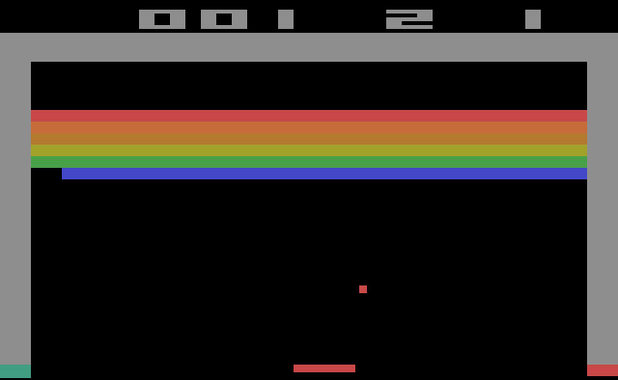
\includegraphics[width=0.99\linewidth]{figs/atari_breakout.jpg}
        \caption{Atari Breakout}
        \label{fig:breakout}
    \end{subfigure}%
    \begin{subfigure}{0.5\textwidth}
        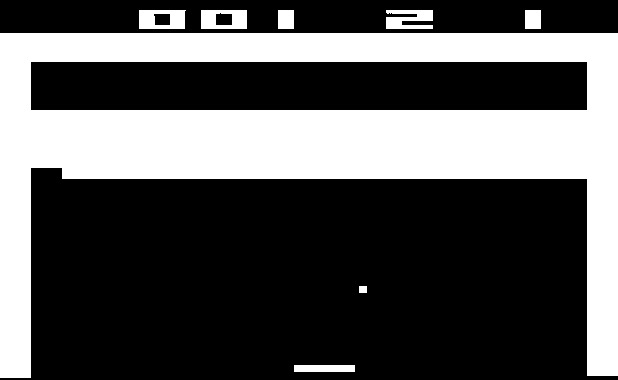
\includegraphics[width=0.99\linewidth]{figs/atari_breakout_bw.jpg}
        \caption{Black and white Breakout}
        \label{fig:bw_breakout}
    \end{subfigure}
    \caption{Atari Breakout. \ref{fig:breakout} is what Breakout looks like. We have the paddle in the bottom of the screen aiming to hit the ball in order to break the tiles at the top of the screen. \ref{fig:bw_breakout} is our transformation of Atari Breakout into black and white pixels for the purpose some of the following problems.}
    \label{fig:my_label}
\end{figure}

% Insert question asking about high state space

% Insert question about tabular is just a special case of linear function approx

% 

\begin{enumerate}
\item \textbf{[1 points]} Suppose we are dealing with the black and white version of Breakout\footnote{Play a Google-Doodle version \href{http://goo.gl/hb5xa}{here}} as in Figure~\ref{fig:bw_breakout}. Furthermore, suppose we are representing the state of the game as just a vector of pixel values without considering if a certain pixel is always black or white. Since we are dealing with the black and white version of the game, these pixel values can either be 0 or 1.

What is the size of the state space?

\begin{tcolorbox}[fit,height=1cm, width=\linewidth, blank, borderline={1pt}{-2pt},nobeforeafter]
%solution
\end{tcolorbox}

    
\item \textbf{[1 points]} In the same setting as the previous part, suppose we wish to apply Q-learning to this problem. What is the size of the Q-value table we will need?

\begin{tcolorbox}[fit,height=1cm, width=\linewidth, blank, borderline={1pt}{-2pt},nobeforeafter]
%solution
\end{tcolorbox}


\clearpage
\item \textbf{[1 points]} Now assume we are dealing with the colored version of Breakout as in Figure~\ref{fig:breakout}. Now each pixel is a tuple of real valued numbers between $0$ and $1$. For example, black is represented as $(0, 0, 0)$ and white is $(1, 1, 1)$. 

What is the size of the state space and Q-value table we will need?

\begin{tcolorbox}[fit,height=1cm, width=\linewidth, blank, borderline={1pt}{-2pt},nobeforeafter]
%solution
\end{tcolorbox}
\end{enumerate}

By now you should see that we will need a huge table in order to apply Q-learning (and similarly value iteration and policy iteration) to Breakout given this state representation. This table would not even fit in the memory of any reasonable computer! Now this choice of state representation is particularly na\"ive. If we choose a better state representation, we could drastically reduce the table size needed. 

On the other hand, perhaps we don't want to spend our days feature engineering a state representation for Breakout. Instead we can apply function approximation to our reinforcement algorithms! The whole idea of function approximation is that states nearby to the state of interest should have \emph{similar} values. That is, we should be able to generalize the value of a state to nearby and unseen states.

Let us define $q_\pi(s, a)$ as the true action value function of the current policy $\pi$. Assume $q_\pi(s,a)$ is given to us by some oracle. Also define $q(s, a; \wv)$ as the action value predicted by the function approximator parameterized by $\wv$. Here $\wv$ is a matrix of size $|\mathcal{S}| \times |\mathcal{A}|$. Clearly we want to have $q(s, a; \wv)$ be close to $q_\pi(s, a)$ for all $(s, a)$ pairs we see. This is just our standard regression setting. That is, our objective function is just the Mean Squared Error:
\begin{align}
J(\wv) = \frac{1}{2} \frac{1}{N} \sum_{s\in\mathcal{S}, a\in\mathcal{A}} \left(q_\pi(s, a) - q(s, a; \wv) \right)^2
\end{align}
Because we want to update for each example stochastically\footnote{This isn't really stochastic, you'll be asked in a bit why.}, we get the following update rule:
\begin{align}
\wv \leftarrow \wv - \alpha \left(q(s, a; \wv) - q_\pi(s,a) \right) \nabla_\wv q(s, a; \wv)
\end{align}

However, more often then not\footnote{Always in real life.} we will not have access to the oracle that gives us our target $q_\pi(s, a)$. So how do we get the target to regress $q(s, a; \wv)$ on? One way is to bootstrap\footnote{Metaphorically, the agent is pulling itself up by its own bootstraps.} an estimate of the action value under a greedy policy using the function approximator itself. That is to say
\begin{align}
q_\pi (s, a) \approx r + \gamma \max_{a'} q(s', a'; \wv)
\end{align}
Where $r$ is the reward observed from taking action $a$ at state $s$, $\gamma$ is the discount factor and $s'$ is the state resulting from taking action $a$ at state $s$. This target is often called the Temporal Difference (TD) target, and gives rise to the following update for the parameters of our function approximator in lieu of a tabular update:

\begin{align}
\wv \leftarrow \wv - \alpha \bigg( \underbrace{q(s, a; \wv) - \underbrace{\big (r + \gamma \max_{a'}q(s', a'; \wv)\big)}_{\text{TD Target}}}_{\text{TD Error}} \bigg) \nabla_\wv q(s, a; \wv)
\end{align}

\begin{enumerate}
\setcounter{enumi}{3}
\item \textbf{[2 points]} Let us consider the setting where we can represent our state by some vector $\sv$, action $a \in \{0, 1, 2\}$ and we choose a linear approximator. That is:
\begin{align}
q(\sv, a; \wv) = \sv^T\wv_a
\end{align}
Again, assume we are in the black and white setting of Breakout as in Figure~\ref{fig:bw_breakout}. Show that tabular Q-learning is just a special case of Q-learning with a linear function approximator by describing a construction of $\sv$. (\textbf{Hint}: Engineer features such that we can encode a table in vector form)

\begin{tcolorbox}[fit,height=4cm, width=\linewidth, blank, borderline={1pt}{-2pt},nobeforeafter]
%solution
\end{tcolorbox}


\item \textbf{[3 points]} Stochastic Gradient Descent works because we can assume that the samples we receive are independent and identically distributed. Is that the case here? If not, why and what are some ways you think you could combat this issue?

\begin{tcolorbox}[fit,height=3cm, width=\linewidth, blank, borderline={1pt}{-2pt},nobeforeafter]
%solution
\end{tcolorbox}


% REMOVING OUT OF SCOPE QUESTION.
% \item \textbf{[2 points]} By bootstrapping the TD error, we are effectively changing our target as we apply gradient descent. This can be an issue as our targets for regression now become extremely noisy. What way(s) do you think could combat this issue.

% \begin{tcolorbox}[fit,height=3cm, width=\linewidth, blank, borderline={1pt}{-2pt},nobeforeafter]
% %solution
% \end{tcolorbox}


\end{enumerate}

